\documentclass[journal,onecolumn,12pt]{IEEEtran}
\IEEEoverridecommandlockouts
% The preceding line is only needed to identify funding in the first footnote. If that is unneeded, please comment it out.
\usepackage{cite}
\usepackage[numbers]{natbib}
\usepackage{amsmath,amssymb,amsfonts}
\usepackage{url}
%\usepackage{algorithmic}
\usepackage{graphicx}
\usepackage{subcaption}
\usepackage{textcomp}
\usepackage{xcolor}
\def\BibTeX{{\rm B\kern-.05em{\sc i\kern-.025em b}\kern-.08em
    T\kern-.1667em\lower.7ex\hbox{E}\kern-.125emX}}

\usepackage[acronym]{glossaries}
% abbreviations:
\newacronym{cnn}{CNN}{Convolution Neural Network}
\newacronym{yolov3}{YOLOv3}{You Look Only Once v3}
\newacronym{hog}{HOG}{Histogram of Oriented Gradients}
\newacronym{surf}{SURF}{Speeded-Up Robust Features}
\newacronym{lbp}{LBP}{Local Binary Patterns}
\begin{document}

\title{The nut job\\
{\footnotesize }%\textsuperscript{*}Note: Sub-titles are not captured in Xplore and should not be used}
%\thanks{Identify applicable funding agency here. If none, delete this.}
}

\author{\IEEEauthorblockN{1\textsuperscript{st} Priteshkumar Gohil}
\IEEEauthorblockA{\textit{Department of Computer Science} \\
\textit{Hochschule Bonn-Rhein-Sieg}\\
Bonn, Germany\\
priteshbgohil@gmail.com}
%\and
%\IEEEauthorblockN{2\textsuperscript{nd} Given Name Surname}
%\IEEEauthorblockA{\textit{dept. name of organization (of Aff.)} \\
%\textit{name of organization (of Aff.)}\\
%City, Country \\
%email address}
%\and
%\IEEEauthorblockN{3\textsuperscript{rd} Given Name Surname}
%\IEEEauthorblockA{\textit{dept. name of organization (of Aff.)} \\
%\textit{name of organization (of Aff.)}\\
%City, Country \\
%email address}
}

\maketitle

\begin{abstract}
Object detection is the task in computer vision to make computer intelligent to recognize and locate the objects. Some of the domains in the object detection are less explored and one such is the food domain. Food packaging industry e.g. peanut packaging service might require to detect bad quality nuts. This paper presents an approach to detect nuts in the scene with cluttered objects, varying illumination condition, and static images. We use \gls{cnn}, a deep learning approach to learn features, classify and localize nuts in the scene. Nuts to detect are peanut, walnut and hazelnut. This paper also presents an algorithm to detect stable frames in the video input, which are based on colour histograms and their difference. The frame detection algorithm can correctly detect the stable frame with an accuracy of 98.94\%. Our deep learning approach can detect nuts in different challenging situations.
\end{abstract}

\begin{IEEEkeywords}
Object Detection, Deep Learning, Event Detection, Convolution Nerual Network
\end{IEEEkeywords}

\section{Introduction}
The visual information that humans and animals perceive has played an important role in interacting with their environment. Giving such capabilities to machines and computer to extract the information of interest from the image helped many sectors like healthcare, driving, robotics, food and beverage etc. Therefore, extracting information of interest from images is the central focus of this project.

Computer vision addressed the problem of automatically extracting useful information from images such as segmentation, classification and object detection, pattern recognition, and many more. One of the active fields of research is object detection aiming to find the answer of two questions. 1. Which objects are in the image, also known as classification and 2. Where objects are located in the image, also known as localization.

Objects in the image are classified based on the features extracted from the bounding box. Figure \ref{fig:original_image_73} and \ref{fig:annotated_image_73_bb} shows the original image and ground truth bounding box. The motivation for selecting features and not pixels for the classification are many. First, features extracted from the object of interest can encode the domain knowledge with finite data. Second, object detection process is faster while using feature based system \cite{Viola2001}. Some of the widely used feature extraction techniques include, \gls{hog} \cite{Dalal2005}, \gls{surf} \cite{Herbert2006}, haar wavelet \cite{Viola2001} and convolution using \gls{cnn} \cite{Alex2012}.
\begin{figure*}
   	\centering
   	\begin{subfigure}[b]{0.475\textwidth}
   		\centering
   		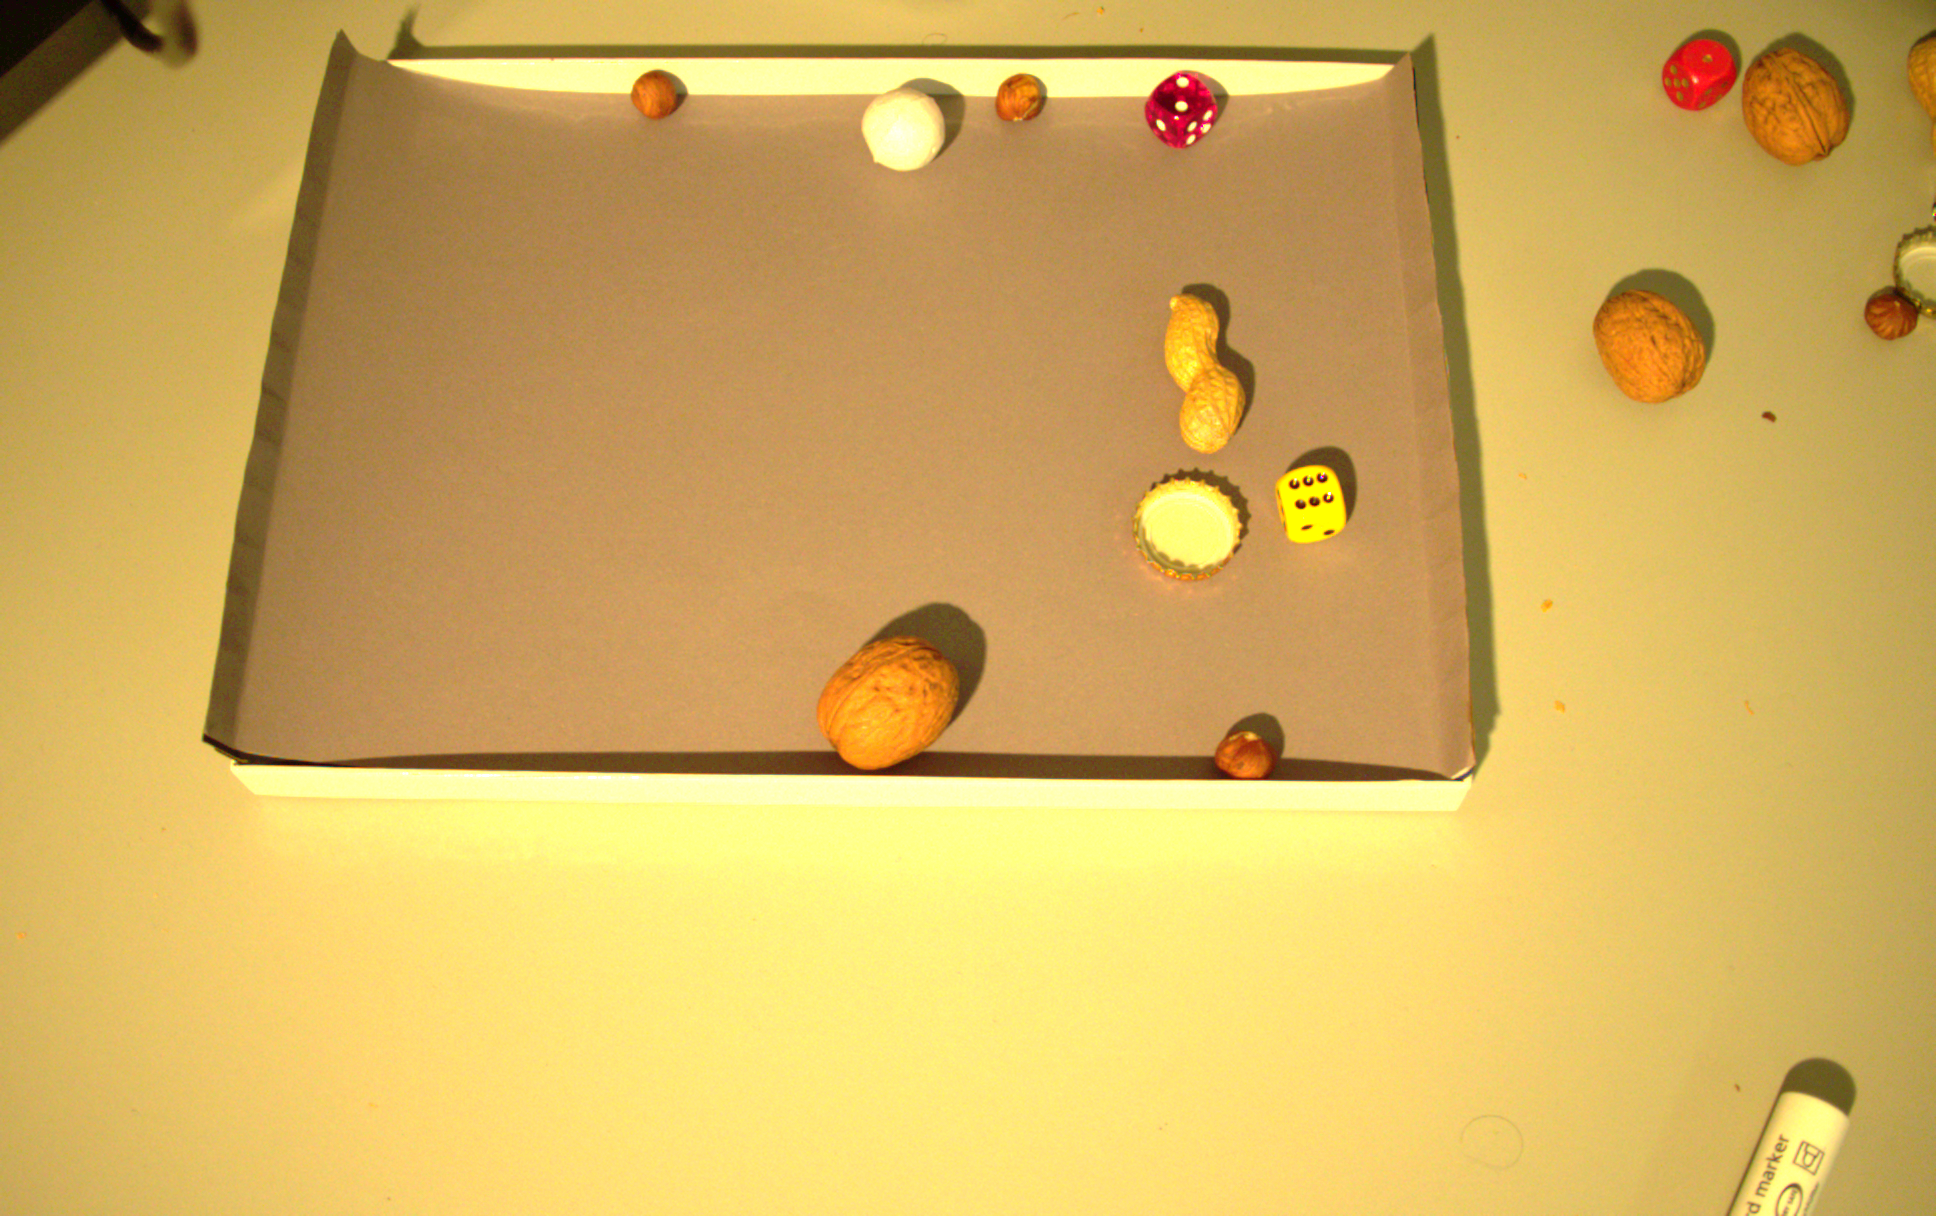
\includegraphics[width=\textwidth]{images/original_image_73}
   		\caption{Image to detect nuts inside the rectangle tray.}
   		\label{fig:original_image_73}
   	\end{subfigure}
   	\hfill
   	\begin{subfigure}[b]{0.475\textwidth}  
   		\centering 
   		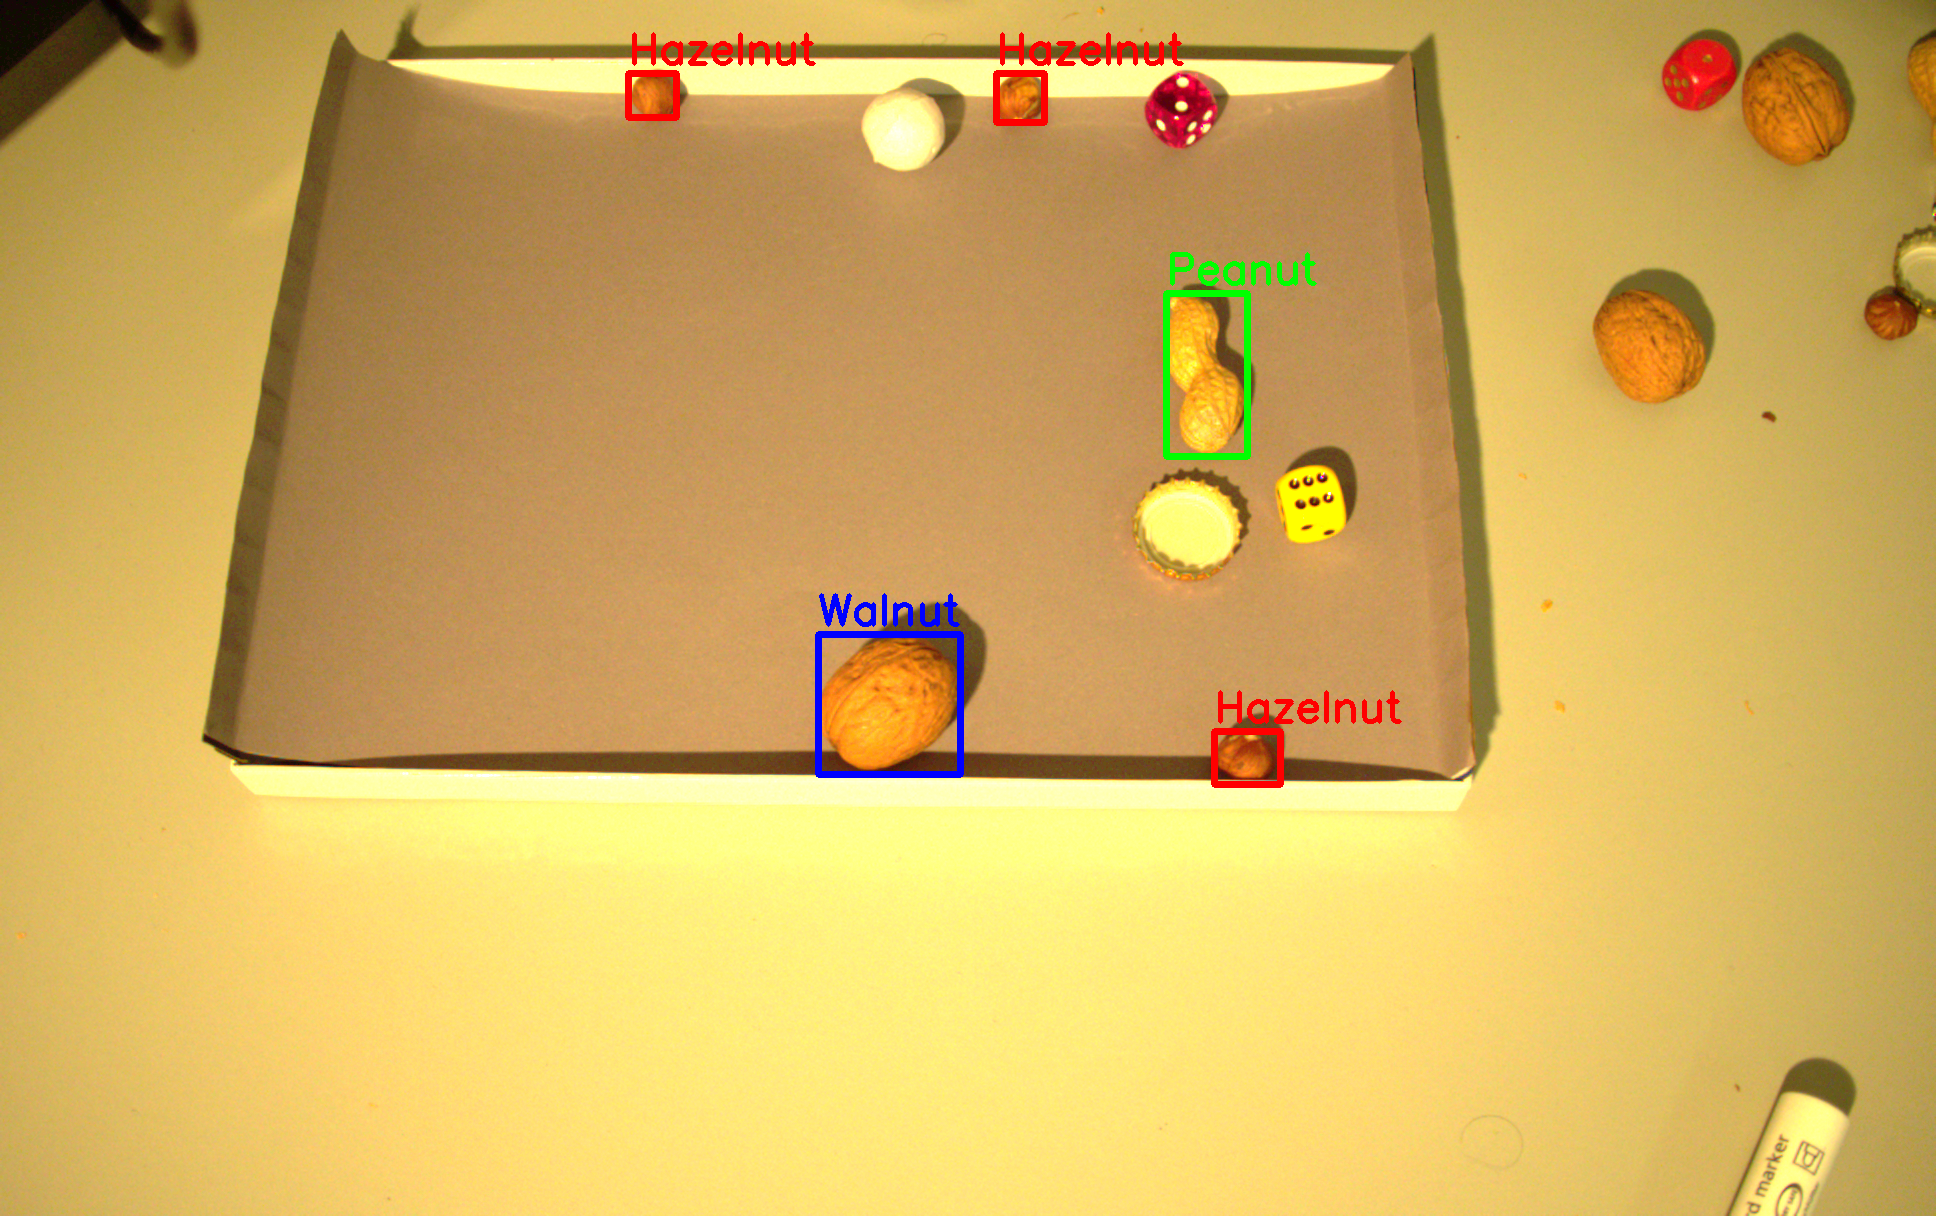
\includegraphics[width=\textwidth]{images/annotated_image_73_bb}
   		\caption{Image annotated with bounding box.}   
   		\label{fig:annotated_image_73_bb}
   	\end{subfigure}
   	\caption{Input image (left) and the ground truth annotation (right) to show the object of interest.}
   	\label{fig:ground_truth}
\end{figure*}

%This report aims to localize the nuts by their center of gravity instead of bounding box. 

%%%% MOTIVATION %%%
%Object detection used in many applications such as...
%Consumption of nuts each year world wide


%%%% PROBLEM STATEMENT %%%%
Detecting objects of interest in the real-world such as peanut, walnut and hazelnut pose different challenging situations. Fundamental characteristic of the nuts is its shape, colour, texture and size. For example, nuts in our experiment shares similar hue but slightly different saturation and value. The texture features of the peanut and walnut can easily be confused by the classifier. Also, shape of peanut might look same but the width and height might vary. Desipte challenges from the object properties, camera and surrounding illumination plays an important role. The camera and the colour information from it impose several challenges. Figure \ref{fig:challenges} illustrates the different challenging situations such as low illumination, high illumination, shadow, occlusion and nuts outside the experimental tray in figure \ref{fig:original_image_73}.
\begin{figure*}
	\centering
	\begin{subfigure}[b]{0.3\textwidth}
		\centering
		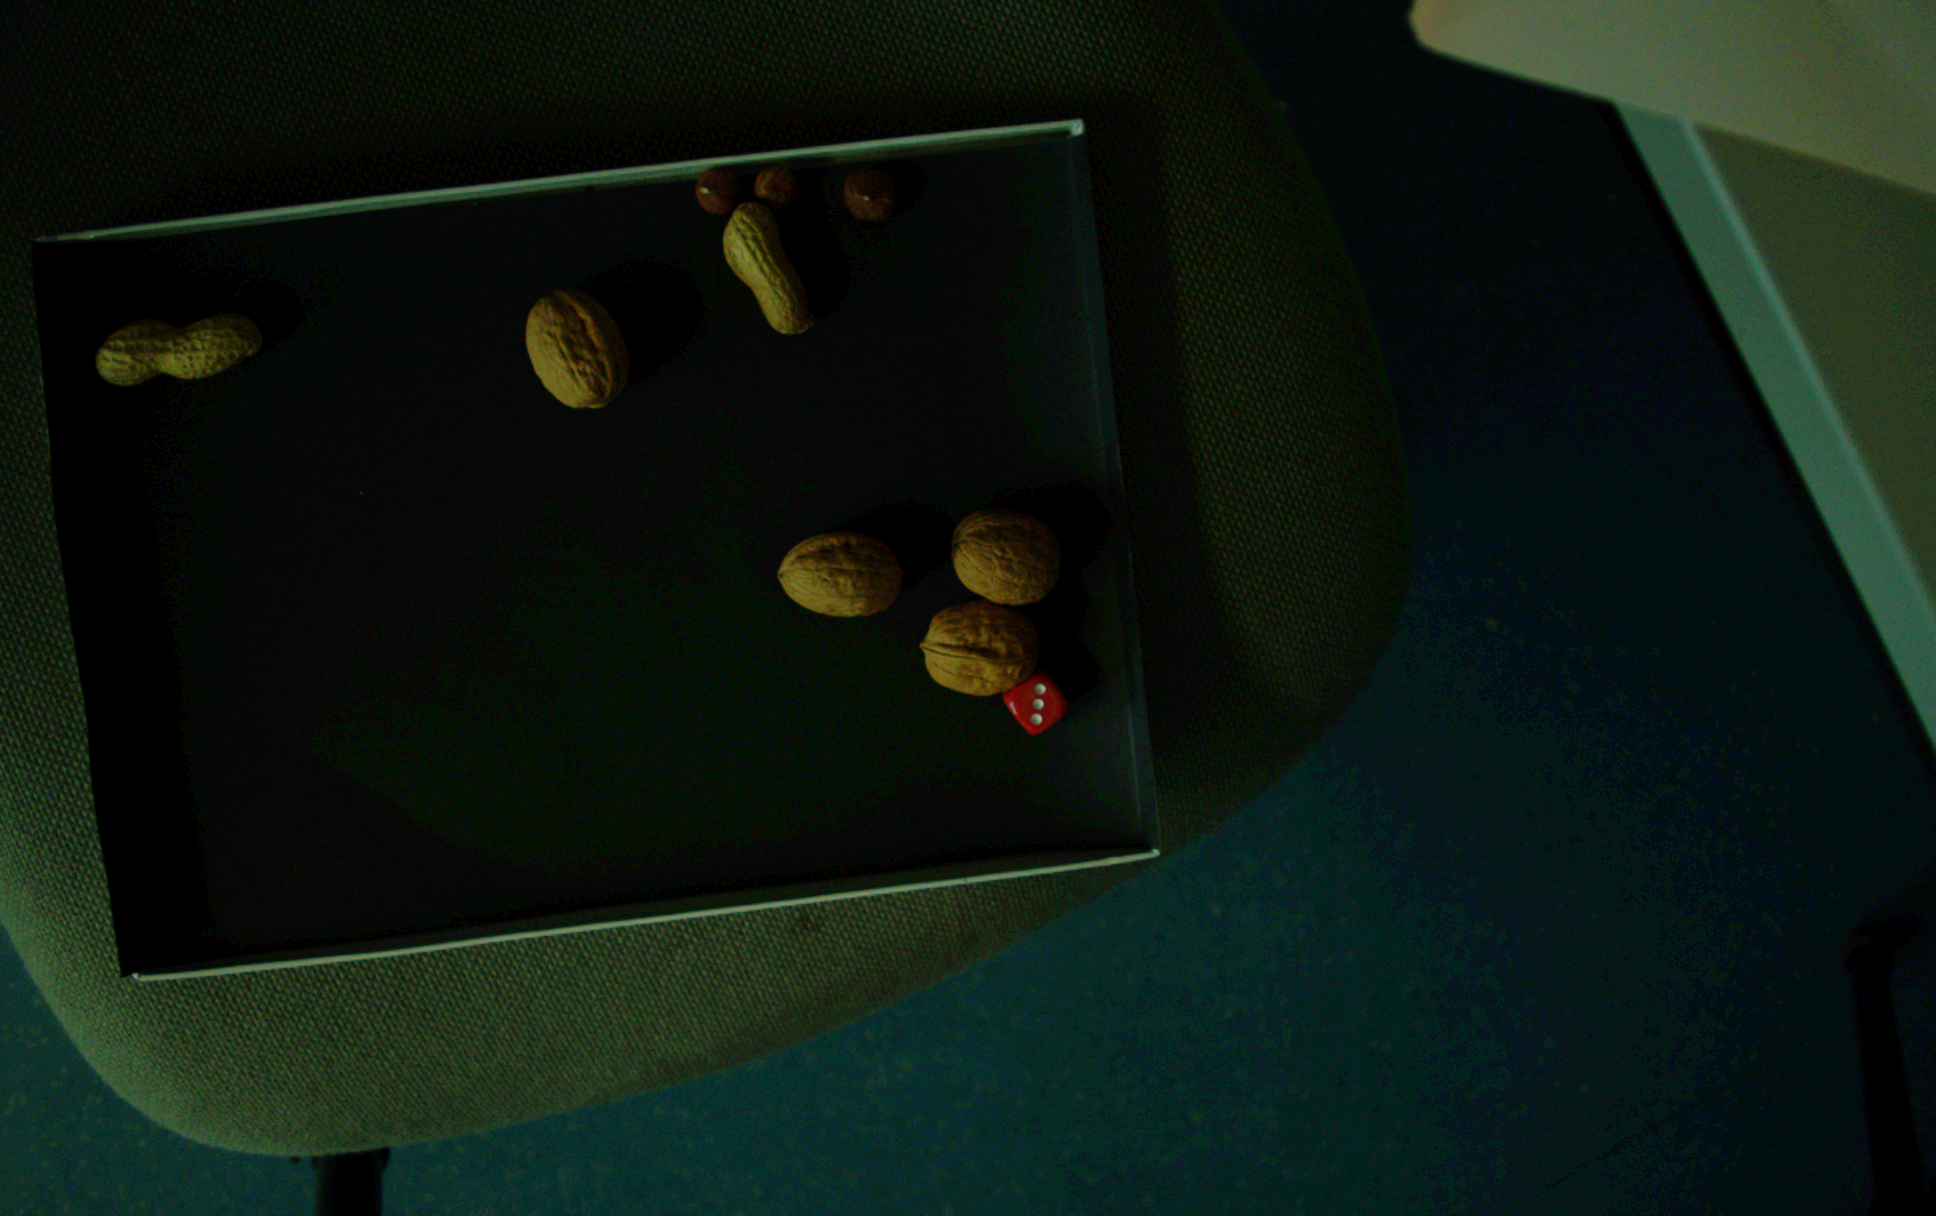
\includegraphics[width=\textwidth]{images/challenges/Low_illu_371.png}
		\caption{Poor illumination}
	\end{subfigure}
	\hfill
	\begin{subfigure}[b]{0.3\textwidth}  
		\centering 
		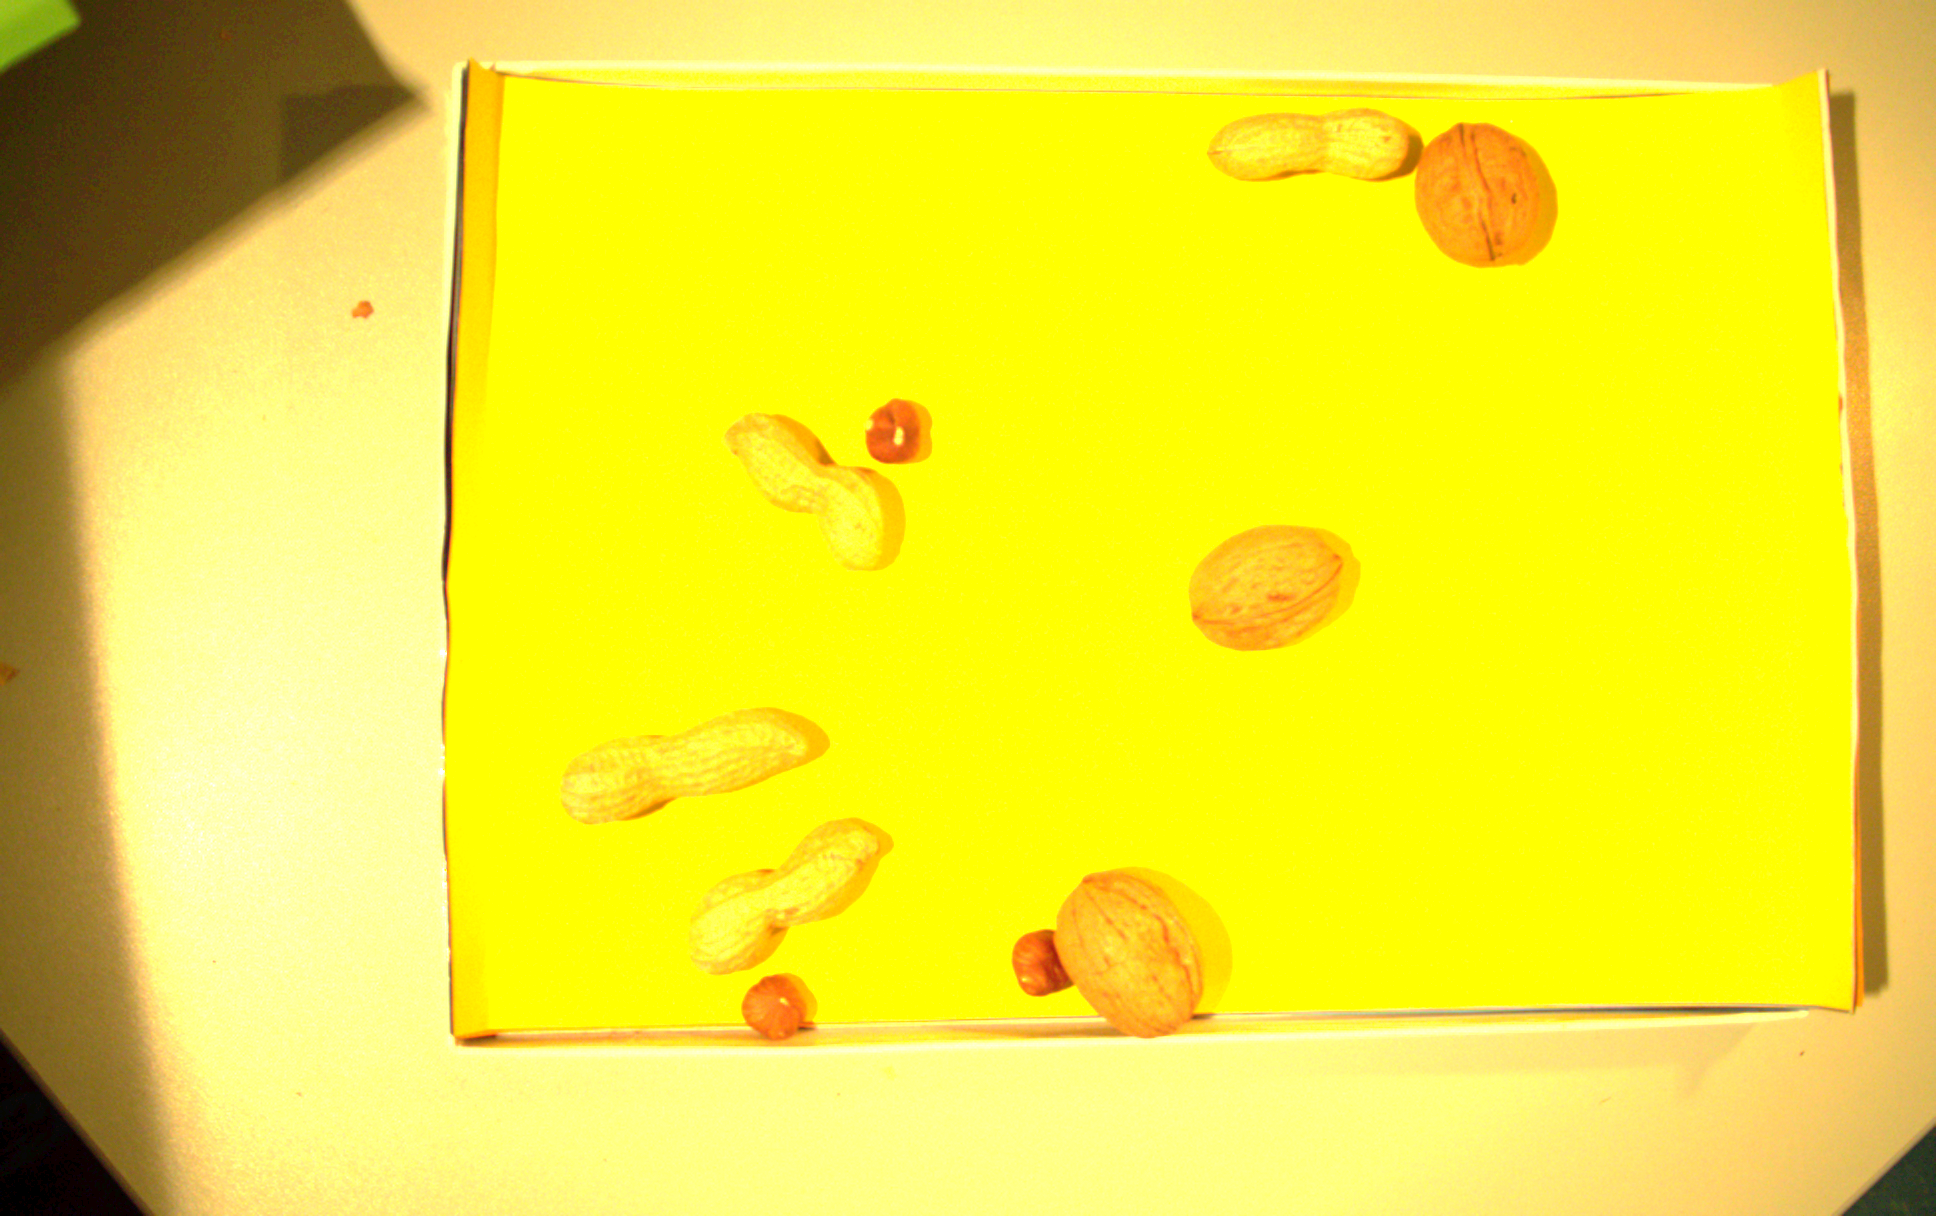
\includegraphics[width=\textwidth]{images/challenges/High_illu_336.png}
		\caption{High illumination} 
	\end{subfigure}
	\hfill
	\begin{subfigure}[b]{0.3\textwidth}  
		\centering 
		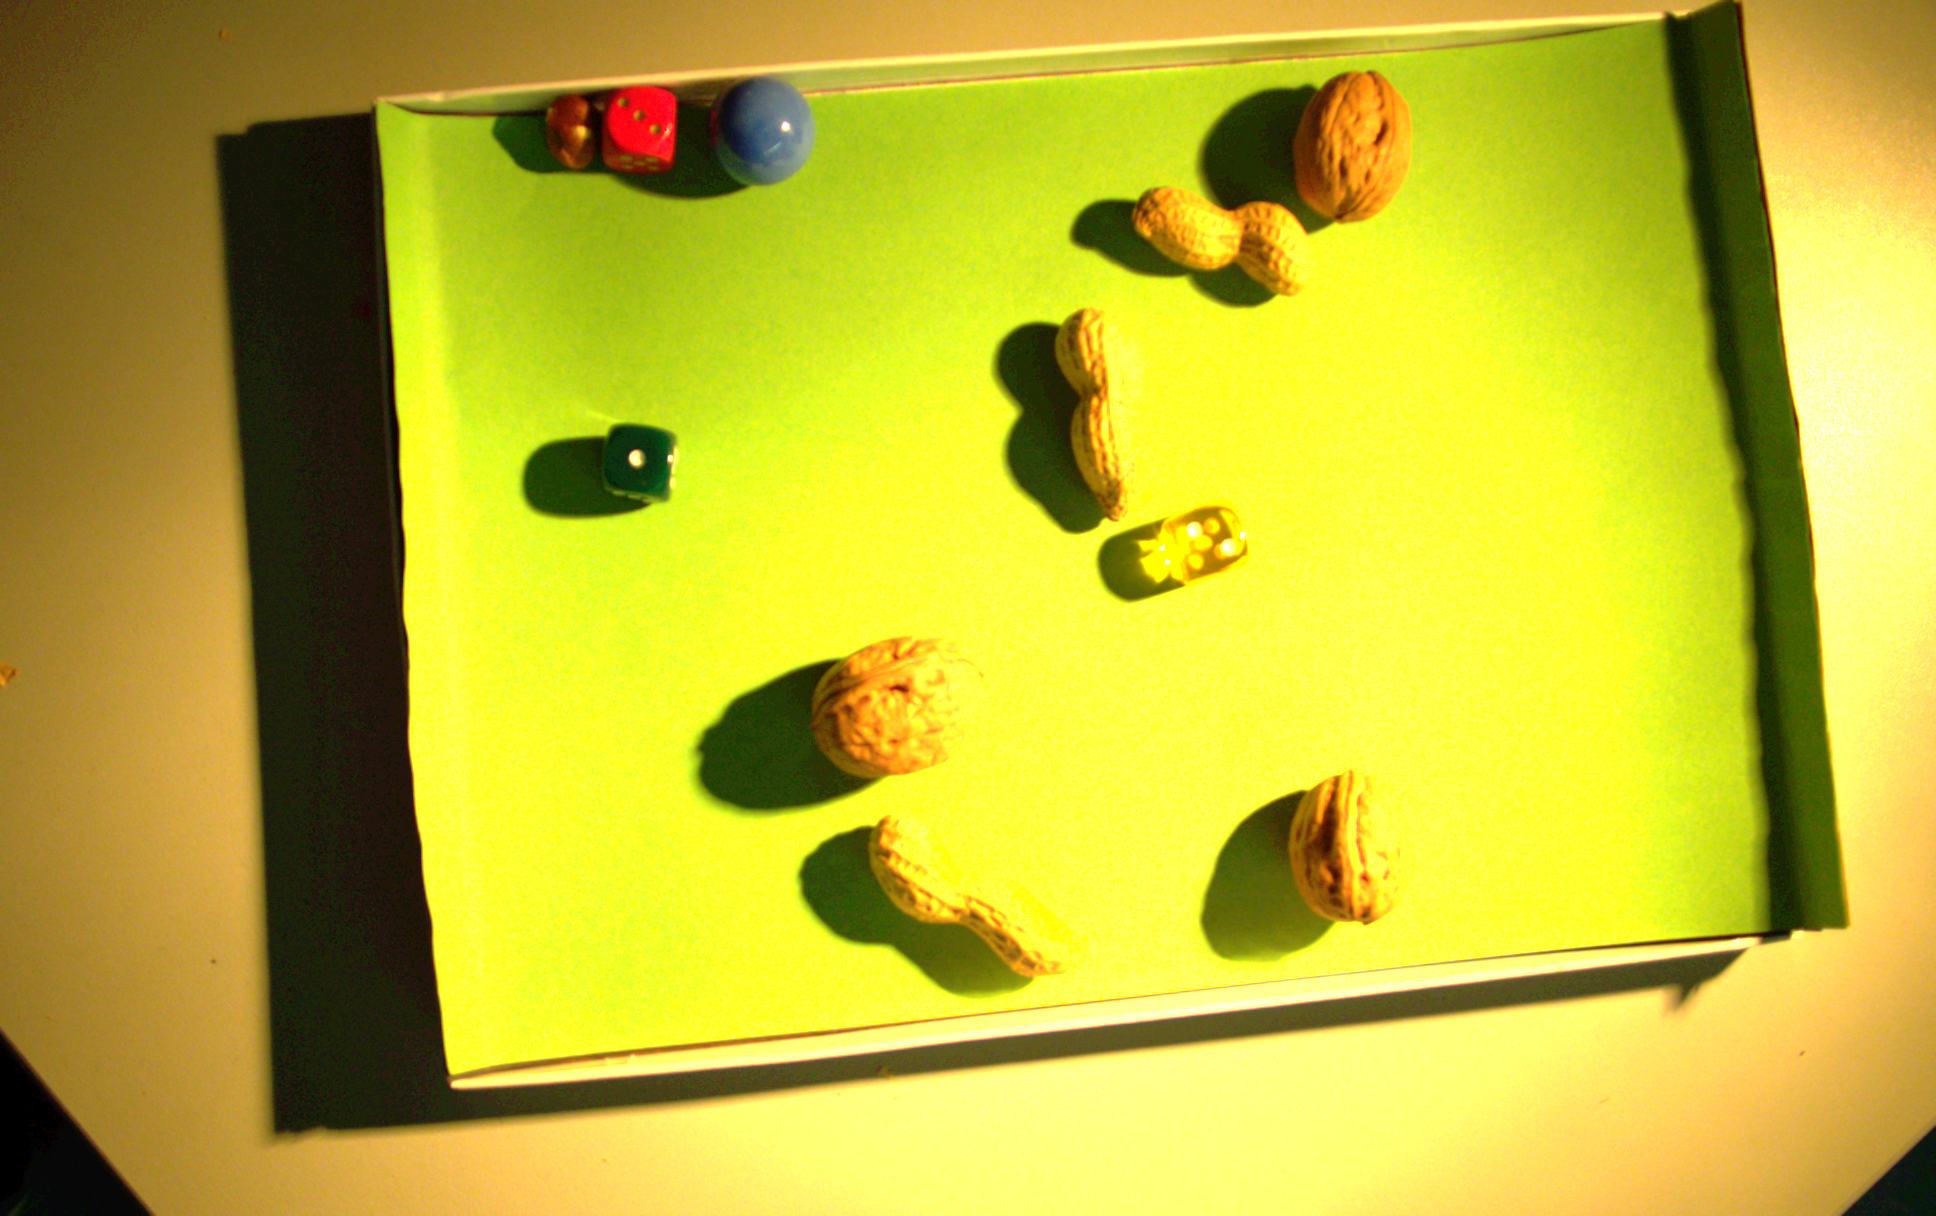
\includegraphics[width=\textwidth]{images/challenges/object_shadow_344.png}
		\caption{Object shadow} 
	\end{subfigure}
	\hfill
	\begin{subfigure}[b]{0.3\textwidth}  
		\centering 
		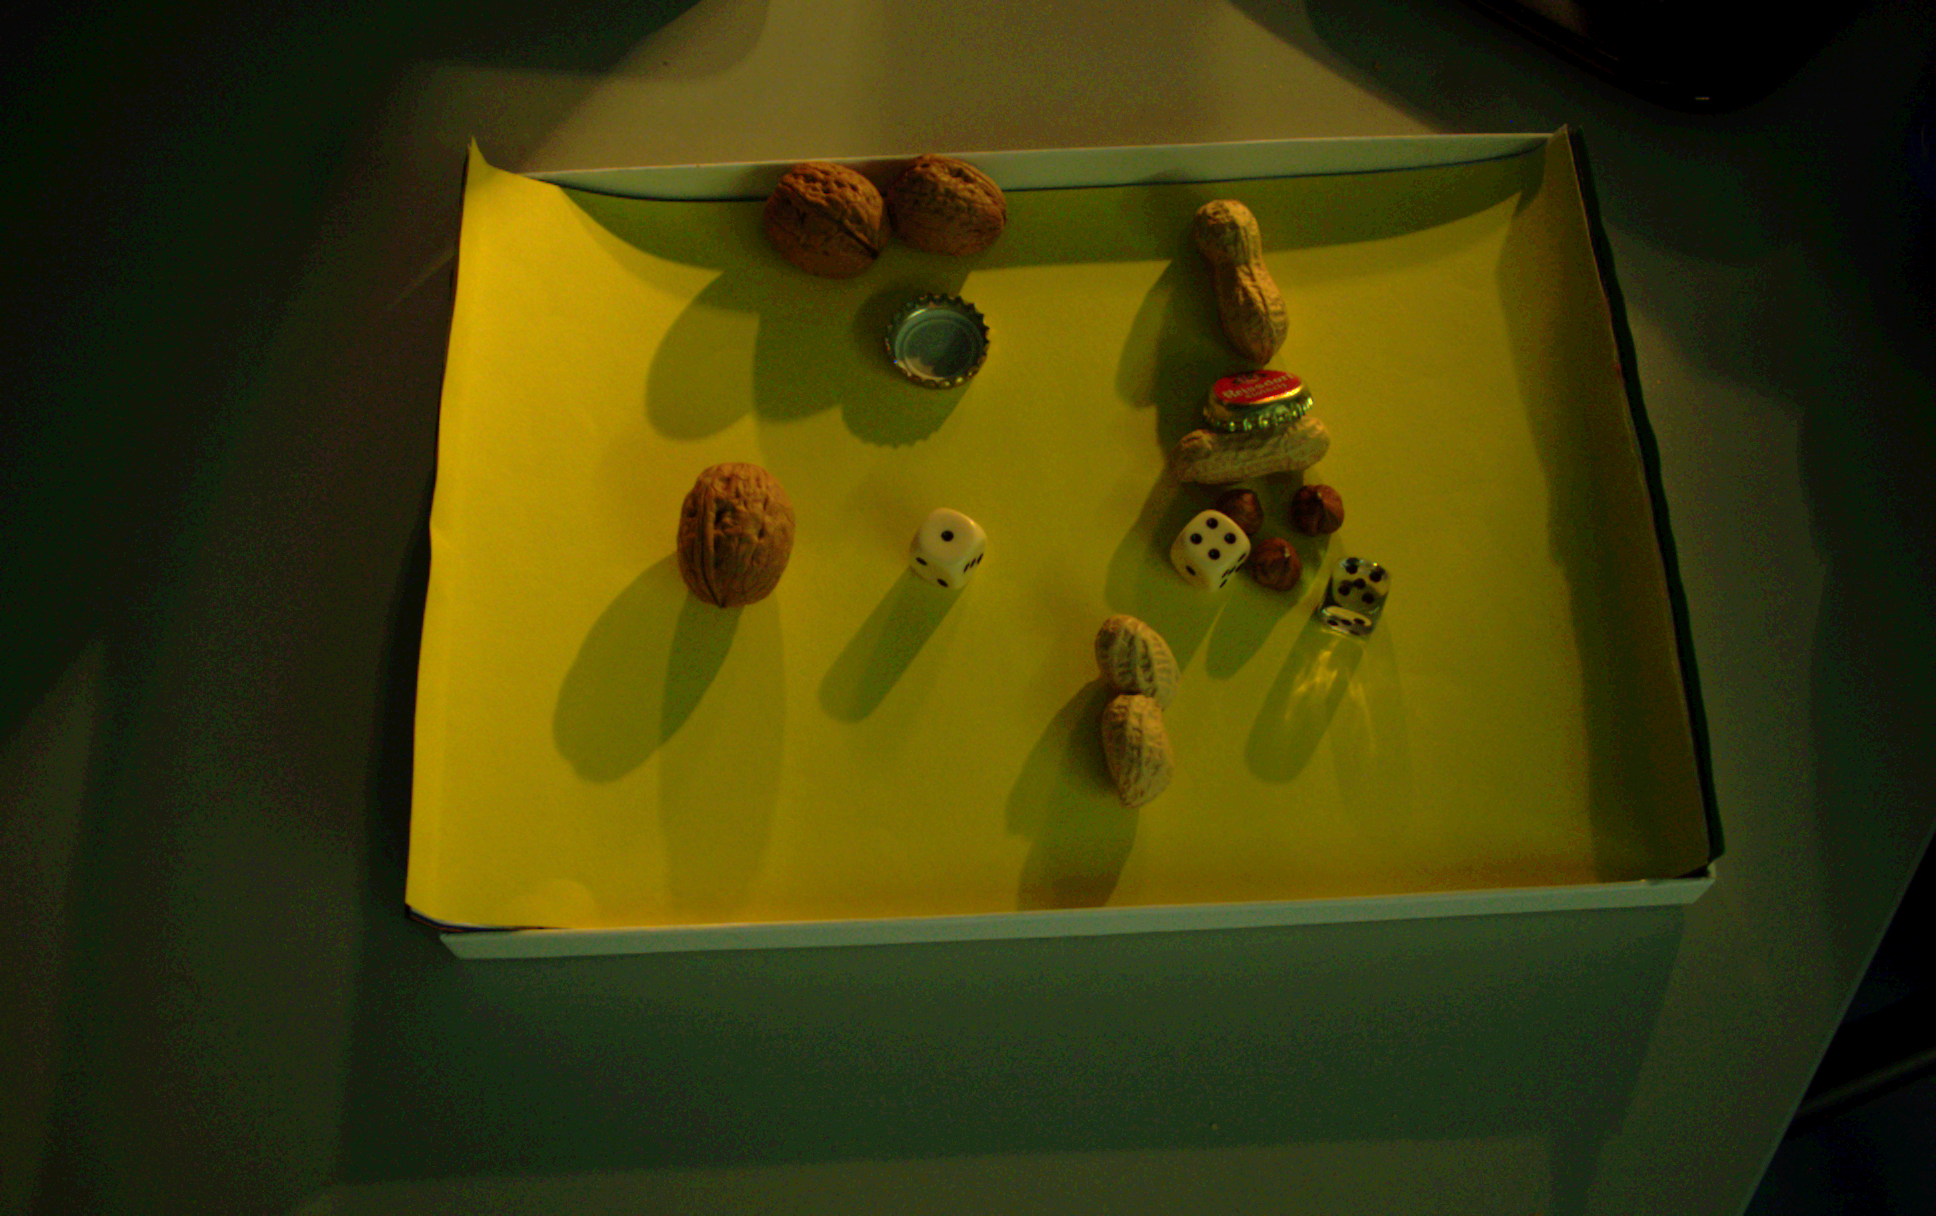
\includegraphics[width=\textwidth]{images/challenges/Cluttered_133.png}
		\caption{Cluttered objects} 
	\end{subfigure}
	\caption{Images from the dataset.}
	\label{fig:challenges}
\end{figure*}


\section{Related works}
Kuo-Yi Huang \cite{Huang2012} detects the areca nuts using computer vision and neural network techniques. Different features such as geometric properties, defect area and colour information are extracted manually. Then Multilayer perceprton is trained on stack of the extracted features to detect the quality. The author is able to detect the areca nuts with 90.9\% accuracy. Similarly, Anita kini et al. \cite{Narendra2018} detects different texture features from gray level co-occurrence matrix (GLCM) to classify type of peanut.

In \cite{Mehdi2019}, deep learning based classifier is designed to detect the quality of pistachios. They use encoder-decoder (autoencoder) structure, where input is first encoded to hidden compressed representation and decoder will try to reproduce an image from the compact hidden representation. They are able to detect bad quality pistachios from oily and darsk stain with an accuracy of 80.3\%. However, their approach is not explaining enough about training data and limited to detect only pistachio.



\section{Material and Methods}
\subsection{Video acquisition}
Videos for the dataset was captured in computer vision lab using machine vision system. The system includes camera connected to the computer. A program is written using OpenCV library to capture the video and stable video frame. Each video frames are of $1936 \times 1216$ pixels and stored in .avi format. Each nuts in the stable frame is annotated with polygon and label using \textit{labelme}\footnote{\url{https://github.com/wkentaro/labelme}} tool. Annotations are saved in JSON format. Figure \ref{fig:bb_image3} shows the annotation mask on the image with the label of each nuts of interest. Note that only single captured video frame is annotated. We have a total of 380 experiments containing videos, images, and annotations file.
\begin{figure}[h]
	\centering
	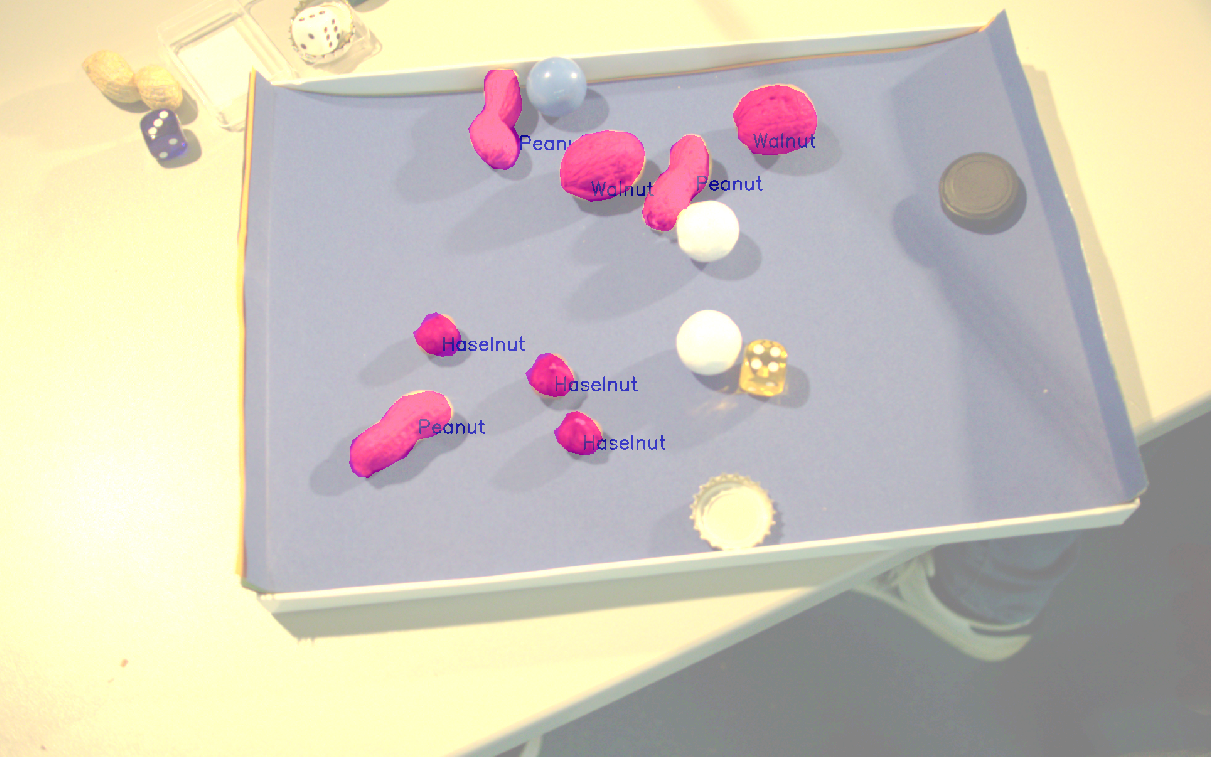
\includegraphics[width=0.5\textwidth]{images/bb_image3}
	\caption{Image with polygon annotation mask and label.}
	\label{fig:bb_image3}
\end{figure}

\subsection{Development tools}
Following tools and systems are used to detect the nuts in our approach.
\begin{itemize}
	\item \textbf{Operating system:} Ubuntu 16.04
	\item \textbf{Programming language:} Python v3.6
	\item \textbf{Deep learning framework:} Pytorch
	\item \textbf{Training model:} University cluster\footnote{\url{https://wr0.wr.inf.h-brs.de/}} 
	\item \textbf{Testing model:} On Windows 10 and Ubuntu 16.04
	\item \textbf{Executable generator:} Pyinstaller
\end{itemize}

\subsection{Proposed approach}
Figure \ref{fig:TTphase} shows the training and testing phase of nut detection. Each module in the training and testing phase is discussed.  
\begin{figure}[h]
	\centering
	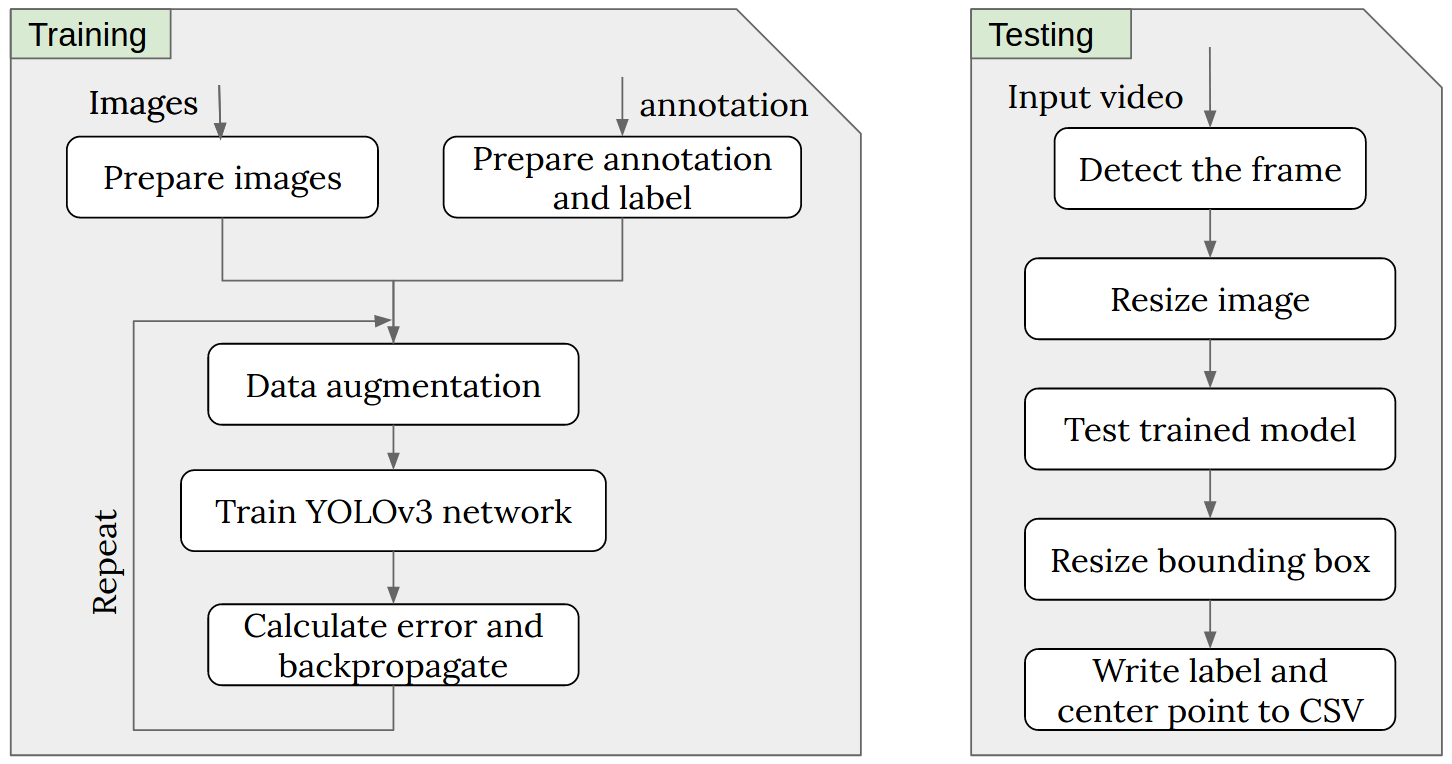
\includegraphics[width=0.7\textwidth]{images/TTphase.png}
	\caption{Training and testing phase of the nuts detection.}
	\label{fig:TTphase}
\end{figure}

\subsubsection{\textbf{Training}} 
\textbf{\newline Images and annotation :} Annotated images are being used to train the network because ground truth is very important for training. To prepare training pipeline, each images are resized to $416 \times 264$ and stored in separate folder. One of the reason to specific resize is the input requirement for \gls{yolov3} and maintaining aspect ration. Whereas, bounding box for each object is extracted from the annotation file, it was normalized and stored in the text file. Each image have label file containing name of the nut, $x$, $y$, $width$ and $height$. We split a total of 380 experiments into 80:20 split and have 304 training data and 76 test data.
\textbf{\newline Data augmentation :} Randomly selected input images and bounding boxes are flipped horizontally. Since our dataset contains all the types of variation, we believe that additional augmentations are not required. However, adding other augmentation techniques is the work we would like to do in the future.
\textbf{\newline Feature extraction and classification :} We use \gls{yolov3}\cite{Joseph2018}, a state of the art architecture to detect the nuts. The architecture of \gls{yolov3} can be seen in the figure \ref{fig:yoloArchitecture}. 
\begin{figure}[h]
	\centering
	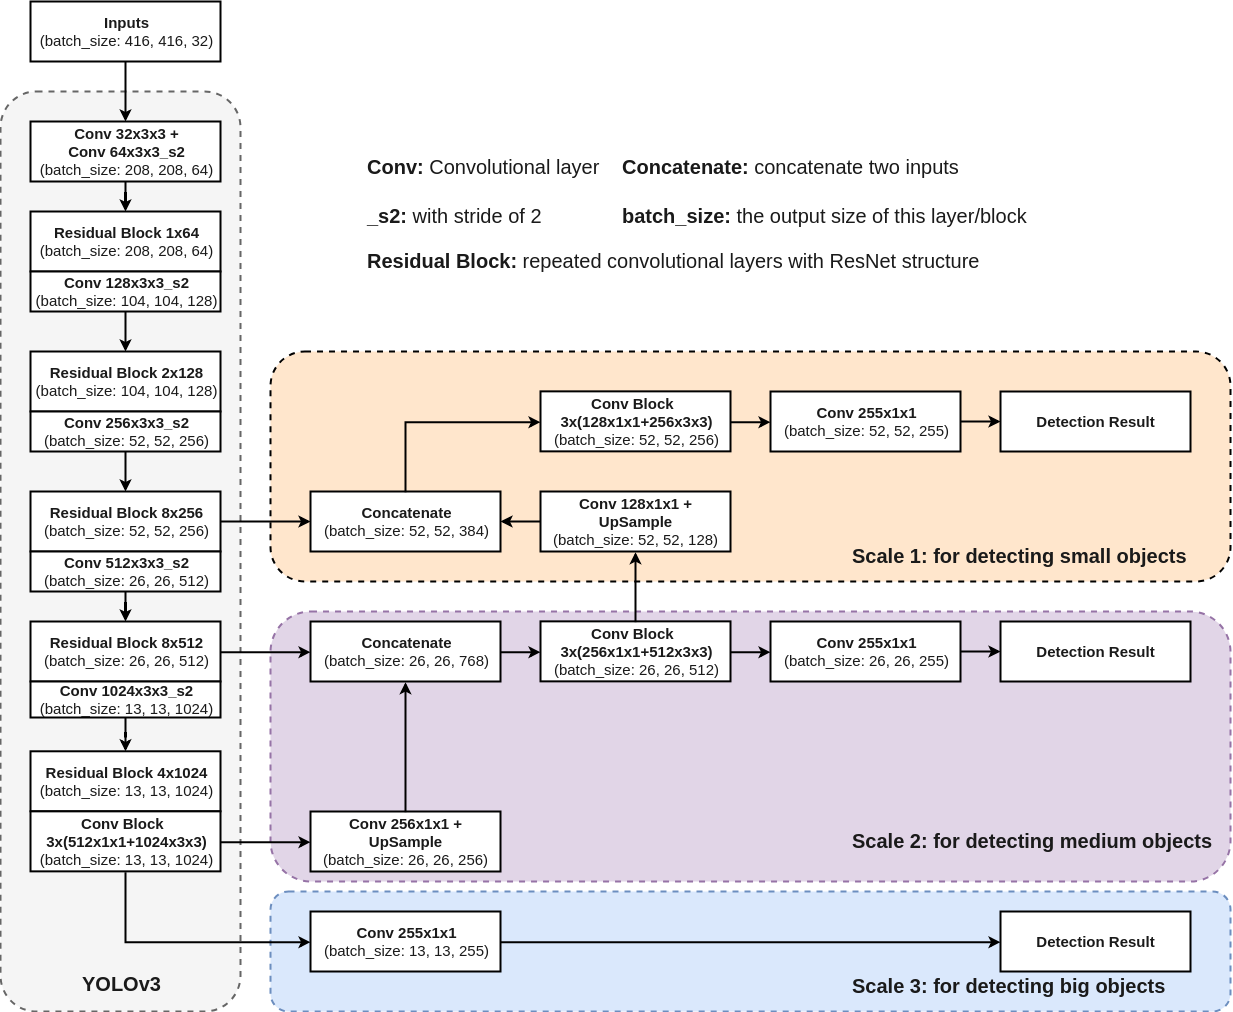
\includegraphics[width=0.8\textwidth]{images/YOLOv3_architecture.png}
	\caption{Architecture of YOLOv3 (image reproduced from \cite{yoloArch}).}
	\label{fig:yoloArchitecture}
\end{figure}
The maximum input size accepted is $416 \times 416 \times 3$. It contains a total of 53 convolution layers. Features from the last convolution layers are flattened and passed through the fully connected layers. Final layer contains 7 neurons in which four values are for bounding box to localize the object, one for confidence of detection and three for each nuts to classify. We have selected batch size of 10 and trained for 900 epoch.
\textbf{\newline Error calculation :} Binary cross entropy loss function is used for multiclass binary classification. And mean square error is used to calculate localization error.
\subsubsection{\textbf{Testing}}
Our testing phase directly accepts the video input and detects the stable frame with nuts. Detected frame then resized to detect objects using trained model. The output bounding box is then resized to actual input image size and the center point of each bounding box with label is written in specified format in CSV file.
\textbf{\newline Stable frame detection :} The stable frame in the video is detected by calculating colour histogram. Figure \ref{fig:detectFrame} shows the flow chart of frame detection algorithm. This algorithm works with an assumption that stable frame is in the first 40\% of the video frames. The colour histogram of current and previous frame is calculated using OpenCV function cv2.calcHist(). Then difference between two histogram is calculated with two different metrics, correlation difference (cv2.HISTCMP\_CORREL) and KL divergence difference (cv2.HISTCMP\_KL\_DIV). Figure \ref{fig:Chistogram} shows the difference of two colour histogram over the entire video. So we try to detect the threshold where KL\_DIV difference is crossing the CORREL difference in first 40\% of frames. The flat region in the KL\_DIV difference shows the stable frames. If the threshold is crossing after 40\% of frames as can be seen in the figure \ref{fig:brightDetect}, KL\_DIV difference is amplified by the factor of 10. This process is repeated until the threshold crosses or 20 iteration, whichever is first. Therefore, we obtain the brown vertical line indicating first highest change in the video. We add offset of 12 to get stable frames (green verical line) which works for most of the video in our dataset. 

\begin{figure*}[h]
	\centering
	\begin{subfigure}[b]{0.55\textwidth}
		\centering
		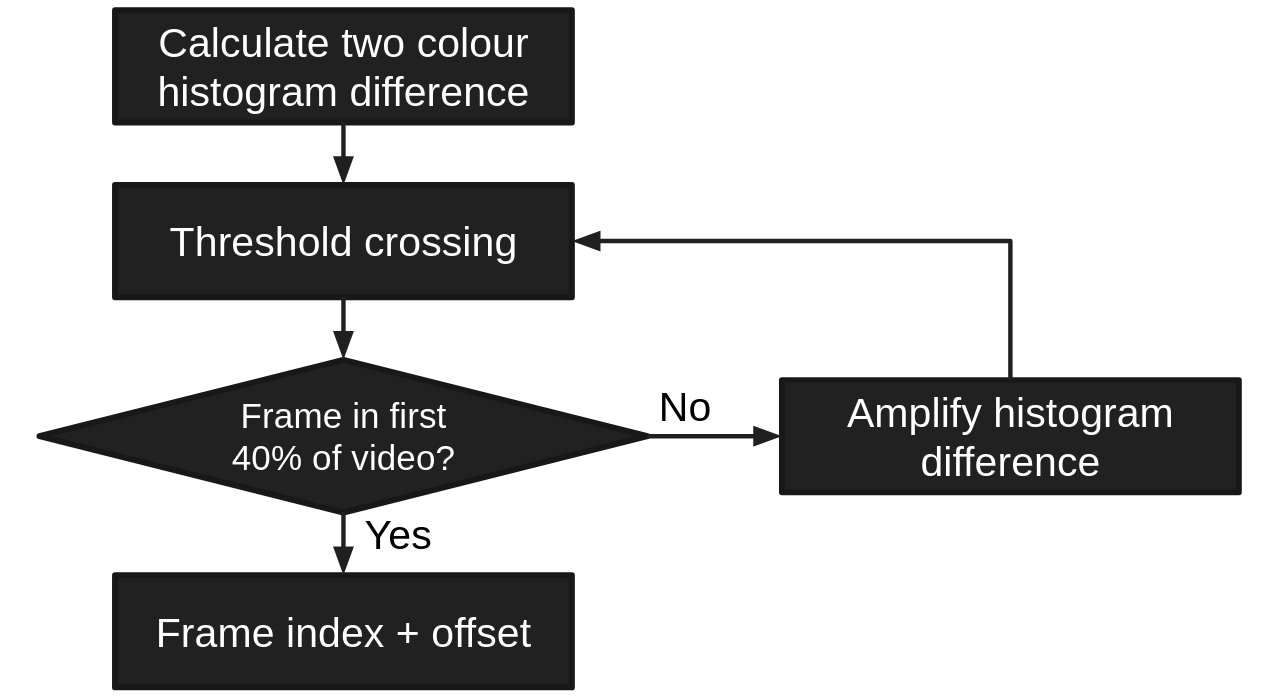
\includegraphics[width=\textwidth]{images/detectFrame.png}
		\caption{Flowchart of stable frame detection algorithm.}
		\label{fig:detectFrame}
	\end{subfigure}
	\begin{subfigure}[b]{0.35\textwidth}  
		\centering 
		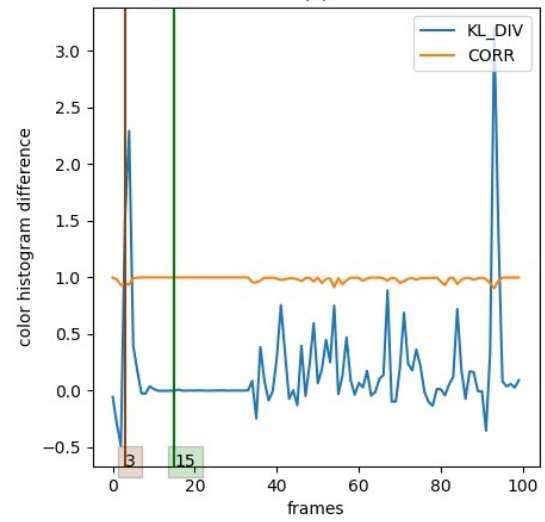
\includegraphics[width=\textwidth]{images/Chistogram.png}
		\caption{Plot of histogram difference.}   
		\label{fig:Chistogram}
	\end{subfigure}
	\caption{Frame detection algorithm (left) and colour histogram difference for video\#3 (right).}
	\label{fig:stableframeAlgo}
\end{figure*}

%Intro: Gentle start with basic terminology
%Problem statement: Still unsolved because of number of challenges. Give images of occlusion, shadow, illumination, . Challenge is takes more time.
%Motivation : Object detection is used in our daily life. Give many examples.
%Proposed approach: Two stage: frame detection and object detection.
%Explain Frame detection
%Explain Object detection
%
%
%Frame detection: 
%perfect situation - 267, 303, 316
%low illumination - 282, 371, 12
%High illumination - 336
%shadow - 315

\section{Results}
Some of the results of a frame detection algorithm is shown in the figure \ref{fig:fd}. Whereas, results of the object detection on test data is shown in figure \ref{fig:resultOD}.
\begin{figure*}[h]
	\centering
	\begin{subfigure}[b]{1\textwidth}
		\centering
		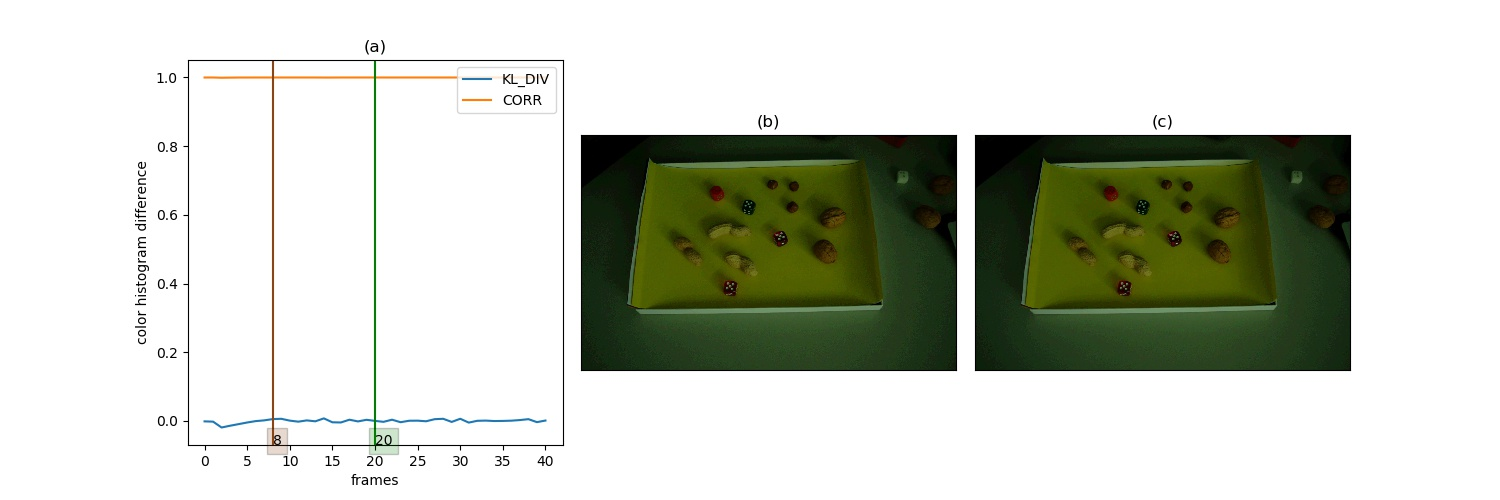
\includegraphics[width=\textwidth]{images/frameDetection/fd_371.jpg}
		\caption{Detecting stable frame in low illumination condition video\#371.}
		\label{fig:darkDetect}
	\end{subfigure}
	\begin{subfigure}[b]{1\textwidth}  
		\centering 
		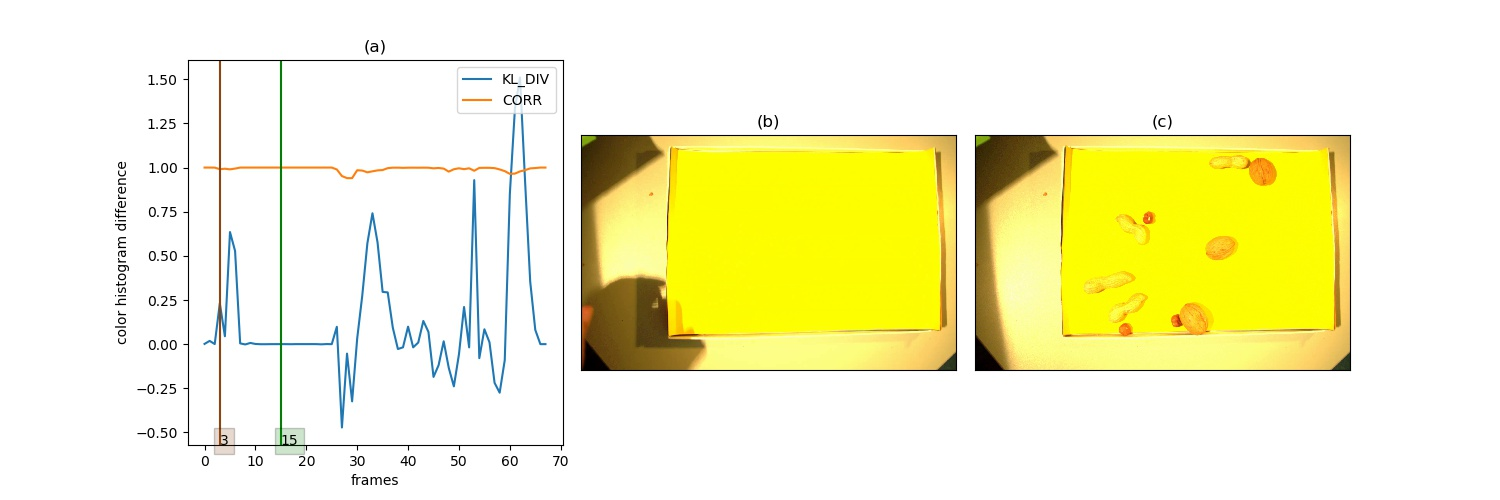
\includegraphics[width=\textwidth]{images/frameDetection/fd_336.jpg}
		\caption{Detecting stable frame in high illumination condition video\#336.}   
		\label{fig:brightDetect}
	\end{subfigure}
	\caption{Frame detection examples.}
	\label{fig:fd}
\end{figure*}

\begin{figure*}
	\centering
	\begin{subfigure}[b]{0.4\textwidth}
		\centering
		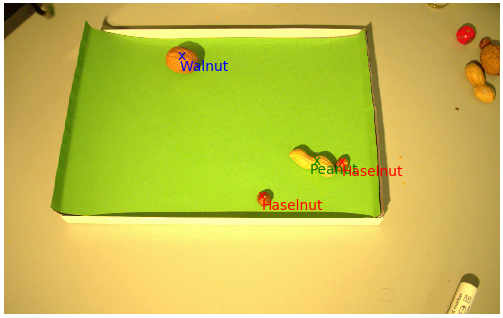
\includegraphics[width=\textwidth]{images/od/perfect_70.png}
%		\caption{Flowchart of stable frame detection algorithm.}
%		\label{fig:}
	\end{subfigure}
	\begin{subfigure}[b]{0.4\textwidth}  
		\centering 
		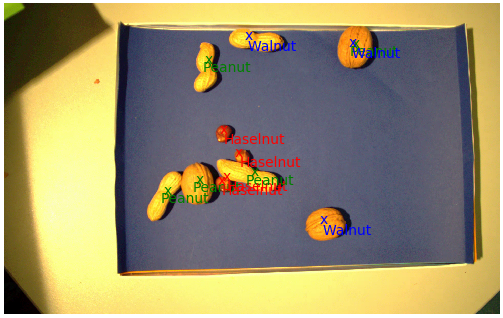
\includegraphics[width=\textwidth]{images/od/CV19_video_337.png}
%		\caption{Plot of histogram difference.}   
%		\label{fig:}
	\end{subfigure}
	\begin{subfigure}[b]{0.4\textwidth}  
		\centering 
		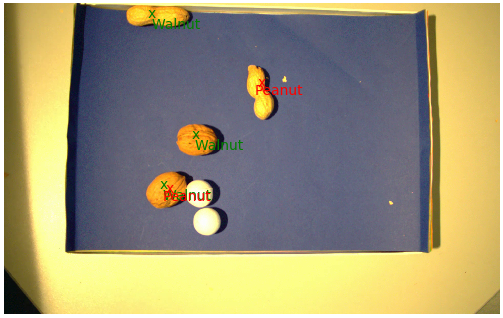
\includegraphics[width=\textwidth]{images/od/missclass_41.png}
		%		\caption{Plot of histogram difference.}   
		%		\label{fig:}
	\end{subfigure}
	\begin{subfigure}[b]{0.4\textwidth}  
		\centering 
		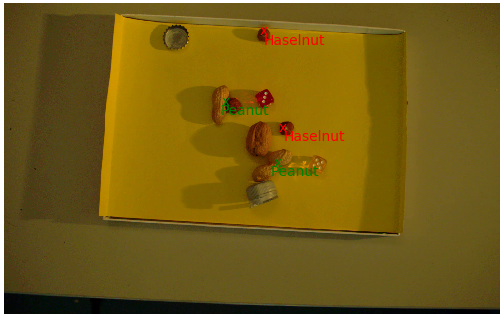
\includegraphics[width=\textwidth]{images/od/missing_353.png}
		%		\caption{Plot of histogram difference.}   
		%		\label{fig:}
	\end{subfigure}
	\caption{Results obtained from trained model on test data.}
	\label{fig:resultOD}
\end{figure*}\goodbreak \newpage

%\subsection{Speed of NN model}
%
%\subsection{stable frame detection}
%
%\subsection{Image processing}
%rescalled, normalized, augmentation
%
%\subsection{Training}
%
%\subsection{Classification results}



\section{\newpage Conclusion}
The nut detection system to detect and localize hazelnut, peanut and walnut is developed in this project. Colour histogram is used to detect the stable frame and deep learning framework is used to detect the nuts in input image. The output of the nut detection system is the pixel value and its label is generated in CSV file. The training was performed with 304 images and 76 videos are used to test the approach. The results on the test data shows that our approach is successfully able to classify the nuts but sometimes it is getting confuse in peanut and the walnut. 

%\section*{Acknowledgment}
%WRITE YOUR ACK here

\newpage
\bibliographystyle{unsrt} % Use the plainnat bibliography style
\bibliography{bibliography.bib} % Use the bibliography.bib file as the source of references
\end{document}
